\chapter{盒子模型与布局模型}

\section{元素分类}

\subsection{我要独占一行——块级元素}

在HTML中\lstinline|<div>|、\lstinline|<p>|、\lstinline|<h1>|、\lstinline|<form>|、\lstinline|<ul>|、\lstinline|<li>|等都是块级元素。每个块级元素都从新的一行开始,并且其后的元素也另起一行。块级元素的高度、宽度、行高遗迹顶和底边距都可以设置,宽度在不设定的情况下,是它本身父容器的100\%(和父元素的宽度一致)。

\begin{lstlisting}[style=htmlcssjs, title=块级元素]
<!DOCTYPE html>
<html lang="en">
<head>
    <meta charset="UTF-8">
    <title>块级元素</title>
</head>
<body>
    <div>这是一个div标签</div>
    <p>这是一个p标签</p>
    <h1>这是一个h1标签</h1>
</body>
</html>
\end{lstlisting}

通过设置\lstinline|display: block|可以将元素显示为块级元素。

\subsection{我要和你站一起——内联元素}

在HTML中,\lstinline|<span>|、\lstinline|<a>|、\lstinline|<label>|、\lstinline|<strong>|、\lstinline|<em>|等都是内联元素(行内元素)。内联元素和其它元素都在一行上,元素的高度、宽度及顶部和底部编剧不可设置,元素的宽度就是它包含的文字或图片的宽度,不可改变。 \\

块级元素也可以设置\lstinline|display: inline|将元素设置为内联元素。

\begin{lstlisting}[style=htmlcssjs, title=内联元素与块级元素转换]
<!DOCTYPE html>
<html lang="en">
<head>
    <meta charset="UTF-8">
    <title>内联元素与块级元素转换</title>
    <style type="text/css">
        a {
            display: block;
        }

        div {
            display: inline;
        }
    </style>
</head>
<body>
    <a>我要变成块级元素</a>
    <a>我也要变成块级元素</a>

    <div>我要变成内联元素</div>
    <div>我也要变成内联元素</div>
</body>
</html>
\end{lstlisting}

\subsection{我还要占个大位置——内联块状元素}

内联块状元素就是同时具备内联元素和块级元素的特点。内联块状元素的特点是和其它元素都在一行上,但元素的高度、宽度、行高以及顶和底边距都可以设置。 \\

通过设置\lstinline|display: inline-block|就可以将元素设置为内联块状元素。如\lstinline|<img>|、\lstinline|<input>|就是这种内联块状标签。

\newpage

\section{盒子模型}

\subsection{盒子模型}

盒子模型包含4个部分:

\begin{enumerate}
    \item 外边距(margin)
    \item 外边框(border)
    \item 内边距(padding)
    \item 内容(content)
\end{enumerate}

\begin{figure}[H]
    \centering
    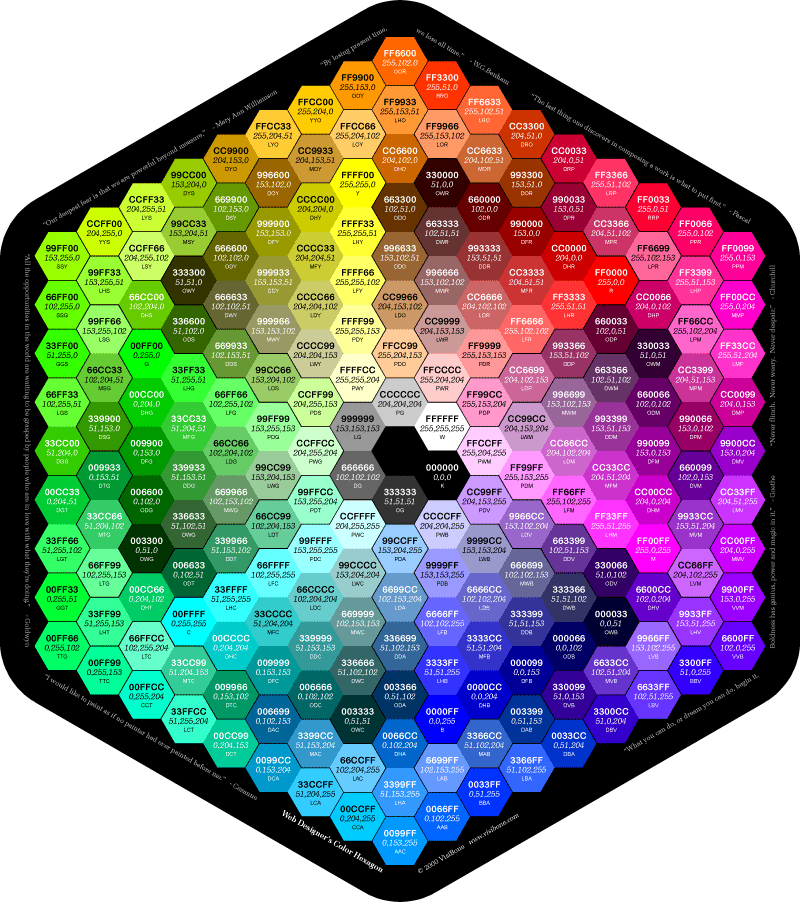
\includegraphics[scale=0.7]{img/C8/8-2/1.png}
\end{figure}

盒模型的宽度和高度和平常所说的物体的宽度和高度的理解是不一样的,CSS内定义的宽和高,指的是盒模型中内容的宽和高。 \\

元素实际的宽度(盒子的宽度) = 左外边距 + 左边框 + 左内边距 + 内容宽度 + 右内边距 + 右边框 + 右外边距 \\

\begin{figure}[H]
    \centering
    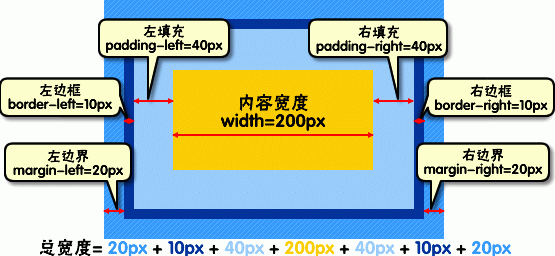
\includegraphics[]{img/C8/8-2/2.png}
\end{figure}

\subsection{外边框(Border)}

盒子模型的外边框可以设置粗细、样式和颜色:

\begin{enumerate}
    \item border-width:设置边框的宽度,常用单位为像素(px)
    \item border-style:边框样式包括实线solid、虚线dashed、点线dotted
    \item border-color:设置边框颜色
\end{enumerate}

当三个属性都需要被设置时,也可以使用border属性简写。例如设置一个粗细为1px实心的黑色边框: \\

\begin{lstlisting}[style=htmlcssjs]
border: 1px solid black;
\end{lstlisting}

CSS中也允许只为一个方向的边框设置属性,使用border-top、border-bottom、border-left、border-right可以单独设置上、下、左、右四条边框。 \\

元素边框的圆角效果可以使用border-radius属性来设置。设置圆角的值的顺序为左上、右上、右下、左下。如果border-radius属性只给出一个值表示四个圆角都被设置成该值。如果只给出两个值表示左上角和右下角设置为第一个值,右上角和左下角设置为第二个值。当给一个正方形的圆角效果值设置为其宽度一半时,显示效果为圆形。

\begin{lstlisting}[style=htmlcssjs, title=圆形]
<!DOCTYPE html>
<html lang="en">
<head>
    <meta charset="UTF-8">
    <title>圆形</title>
    <style type="text/css">
        div {
            width: 100px;
            height: 100px;
            background-color: red;
            border-radius: 50%;
        }
    </style>
</head>
<body>
    <div></div>
</body>
</html>
\end{lstlisting}

通过单独设置每条边的属性,可以在正方形内展现不同的颜色。

\begin{figure}[H]
    \centering
    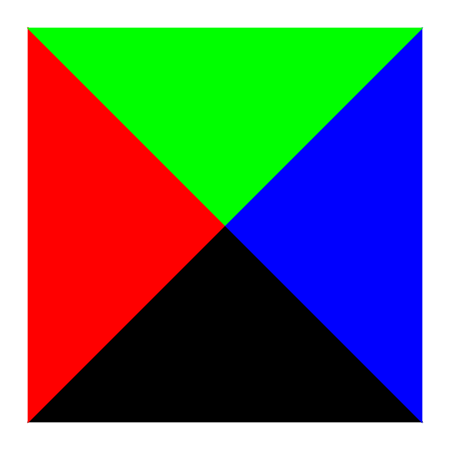
\begin{tikzpicture}
        \filldraw[draw=black, fill=black] (0,0) -- (5,0) -- (2.5,2.5) -- cycle;
        \filldraw[draw=red, fill=red] (0,0) -- (2.5,2.5) -- (0,5) -- cycle;
        \filldraw[draw=blue, fill=blue] (5,0) -- (2.5,2.5) -- (5,5) -- cycle;
        \filldraw[draw=green, fill=green] (2.5,2.5) -- (0,5) -- (5,5) -- cycle;
    \end{tikzpicture}
\end{figure}

\begin{lstlisting}[style=htmlcssjs, title=四色正方形]
<!DOCTYPE html>
<html lang="en">
<head>
    <meta charset="UTF-8">
    <title>四色正方形</title>
    <style type="text/css">
        div {
            width: 0;
            height: 0;
            border: 100px solid black;
            border-left-color: red;
            border-top-color: green;
            border-right-color: blue;
        }
    </style>
</head>
<body>
    <div></div>
</body>
</html>
\end{lstlisting}

通过设置透明色(transparent),可以绘制出三角形。

\begin{figure}[H]
    \centering
    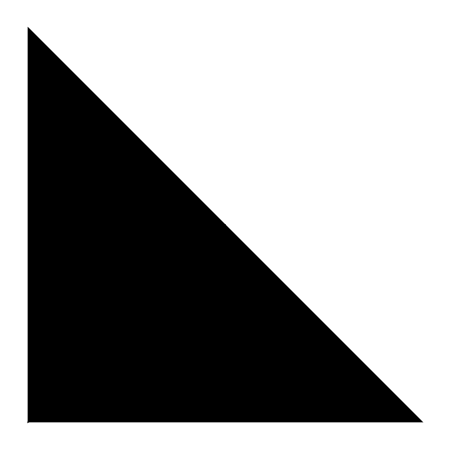
\begin{tikzpicture}
        \filldraw[draw=black, fill=black] (0,0) -- (5,0) -- (2.5,2.5) -- cycle;
        \filldraw[draw=black, fill=black] (0,0) -- (2.5,2.5) -- (0,5) -- cycle;
    \end{tikzpicture}
\end{figure}

\begin{lstlisting}[style=htmlcssjs, title=三角形]
<!DOCTYPE html>
<html lang="en">
<head>
    <meta charset="UTF-8">
    <title>三角形</title>
    <style type="text/css">
        div {
            width: 0;
            height: 0;
            border: 100px solid black;
            border-left-color: black;
            border-top-color: transparent;
            border-right-color: transparent;
        }
    </style>
</head>
<body>
    <div></div>
</body>
</html>
\end{lstlisting}

\subsection{内边距(Padding)}

元素内容与边框之间是可以设置距离的,称之为内边距或填充。内边距也可分为上、右、下、左(顺时针)。

\begin{figure}[H]
    \centering
    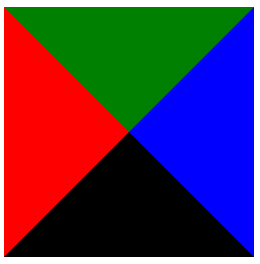
\includegraphics[scale=0.7]{img/C8/8-2/3.png}
\end{figure}

\subsection{外边距(Margin)}

元素与其他元素之间的距离可以使用外边距来设置,外边距也可分为上、右、下、左。

\begin{figure}[H]
    \centering
    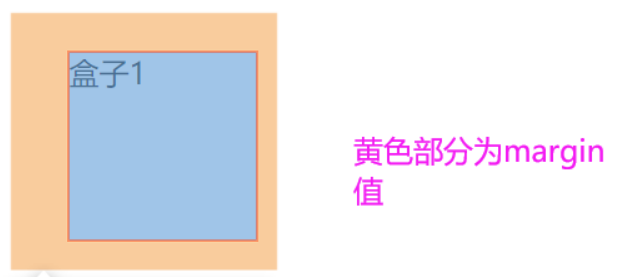
\includegraphics[scale=0.7]{img/C8/8-2/4.png}
\end{figure}

margin与padding的区别在于,padding在外边框里,margin在外边框外。

\newpage

\section{布局模型}

\subsection{布局模型}

布局模型建立在盒子模型的基础上,在网页中,元素有3种布局模型:

\begin{enumerate}
    \item 流动模型(flow)
    \item 浮动模型(float)
    \item 层模型(layer)
\end{enumerate}

\subsection{流动模型}

流动模型是默认的网页布局模式,也就是说网页在默认状态下的HTML网页元素都是根据流动模型来分布网页内容的。 \\

流动布局模型有2个典型的特征:

\begin{enumerate}
    \item 块级元素都会在所处的包含元素内自上而下按顺序垂直延伸分布,因为在默认状态下,块级元素的宽度都为100\%,即都会以行的形式占据位置。
          \begin{figure}[H]
              \centering
              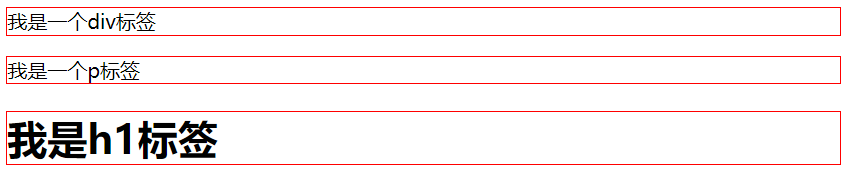
\includegraphics[scale=0.7]{img/C8/8-3/1.png}
          \end{figure}

    \item 内联元素都会在所处的包含元素内从左到右水平分布显示。
          \begin{figure}[H]
              \centering
              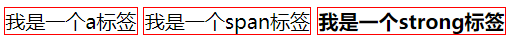
\includegraphics[]{img/C8/8-3/2.png}
          \end{figure}
\end{enumerate}

\subsection{浮动模型}

块级元素这么霸道都是独占一行,如果想让两个块级元素并排显示,可以设置元素浮动。任何元素在默认情况下是不能浮动的,但可以设置float属性定义为浮动,如\lstinline|<div>|、\lstinline|<p>|、\lstinline|<table>|、\lstinline|<img>|等元素都可以被定义为浮动。

\begin{lstlisting}[style=htmlcssjs, title=浮动模型]
<!DOCTYPE html>
<html lang="en">
<head>
    <meta charset="UTF-8">
    <title>浮动模型</title>
    <style type="text/css">
        div {
            width: 100px;
            height: 100px;
            border: 1px solid red;
        }

        #div1 {
            float: left;
        }

        #div2 {
            float: right;
        }
    </style>
</head>
<body>
    <div id="div1"></div>
    <div id="div2"></div>
</body>
</html>
\end{lstlisting}

\newpage

\section{定位}

\subsection{层模型}

层布局模型就像是图像软件PhotoShop中非常流行的图层编辑功能一样,每个图形能够精确定位操作(positioning)。由于有些元素是定点展示的,定位技术可以让元素在特定的位置出现。 \\

层模型有3种形式:

\begin{enumerate}
    \item 绝对定位(absolute)
    \item 相对定位(relative)
    \item 固定定位(fixed)
\end{enumerate}

\subsection{万事无绝对——绝对定位}

如果想为元素设置层模型中的绝对定位,需要设置\lstinline|position: absolute|,这条语句的作用是将元素从文档流中拖出来,然后使用left、right、top、bottom属性相对于其最接近的一个具有定位属性的父包含块进行绝对定位。如果不存在这样的包含块,则相对于body元素,即相对于浏览器窗口。 \\

当一个元素成为绝对定位元素,它就脱离了原来的层面,原来的位置会空出,下面的元素都会上来。

\begin{lstlisting}[style=htmlcssjs, title=绝对定位]
<!DOCTYPE html>
<html lang="en">
<head>
    <meta charset="UTF-8">
    <title>绝对定位</title>
    <style type="text/css">
        div {
            width: 100px;
            height: 100px;
        }

        #div1 {
            background-color: red;
            position: absolute;
            top: 50px;      /* 距离窗口上边50px */
            left: 100px;    /* 距离窗口左边100px */
        }

        #div2 {
            background-color: blue;
        }
    </style>
</head>
<body>
    <div id="div1"></div>
    <div id="div2"></div>
</body>
</html>
\end{lstlisting}

\begin{figure}[H]
    \centering
    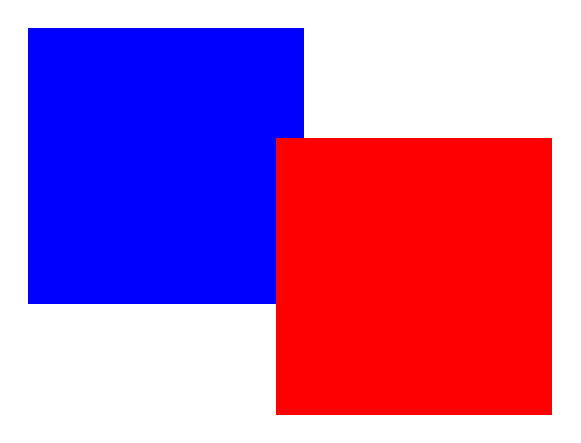
\begin{tikzpicture}[scale=0.7]
        \filldraw[draw=blue, fill=blue] (0,2) -- (0,7) -- (5,7) -- (5,2) -- cycle;
        \filldraw[draw=red, fill=red] (4.5,0) -- (9.5,0) -- (9.5,5) -- (4.5,5) -- cycle;
    \end{tikzpicture}
\end{figure}

\subsection{相对于自己的位置——相对定位}

如果想为元素设置层模型中的相对定位,需要设置\lstinline|position: relative|,它通过left、right、top、bottom属性确定元素在正常文档流中的偏移位置。相对定位完成的过程是首先按static (float)方式生成一个元素,然后相对于以前的位置移动,并且偏移前的位置保留不动,因此下面的元素无法上来。

\begin{lstlisting}[style=htmlcssjs, title=相对定位]
<!DOCTYPE html>
<html lang="en">
<head>
    <meta charset="UTF-8">
    <title>相对定位</title>
    <style type="text/css">
        div {
            width: 100px;
            height: 100px;
        }

        #div1 {
            background-color: red;
            position: relative;
            top: 50px;
            left: 100px;
        }

        #div2 {
            background-color: blue;
        }
    </style>
</head>
<body>
    <div id="div1"></div>
    <div id="div2"></div>
</body>
</html>
\end{lstlisting}

\begin{figure}[H]
    \centering
    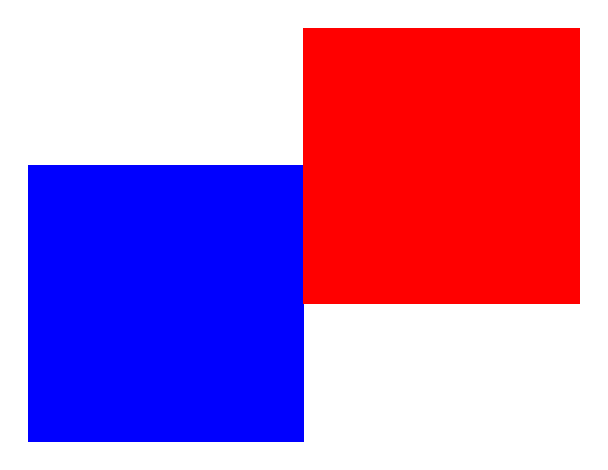
\begin{tikzpicture}[scale=0.7]
        \filldraw[draw=blue, fill=blue] (0,0) -- (0,5) -- (5,5) -- (5,0) -- cycle;
        \filldraw[draw=red, fill=red] (5,2.5) -- (5,7.5) -- (10,7.5) -- (10,2.5) -- cycle;
    \end{tikzpicture}
\end{figure}

使用\lstinline|position: absolute|可以实现元素相对于浏览器(body)设置定位,那可不可以相对于其它元素进行定位呢?当然可以,但是必须要满足以下的3点条件:

\begin{enumerate}
    \item 参照定位的元素必须是相对定位元素的前辈元素。
    \item 参照定位的元素必须加入\lstinline|position: relative|。
    \item 定位元素加入`position: absolute`后便可以使用top、bottom、left、right来进行偏移了。
\end{enumerate}

\begin{lstlisting}[style=htmlcssjs, title=相对父元素定位]
<!DOCTYPE html>
<html lang="en">
<head>
    <meta charset="UTF-8">
    <title>相对父元素定位</title>
    <style type="text/css">
        #div1 {
            width: 100px;
            height: 100px;
            background-color: red;
            position: relative;
        }

        #div2 {
            width: 100px;
            height: 20px;
            background-color: blue;
            position: absolute;
            top: 40px;
        }
    </style>
</head>
<body>
    <div id="div1">
        <div id="div2"></div>
    </div>
</body>
</html>
\end{lstlisting}

\begin{figure}[H]
    \centering
    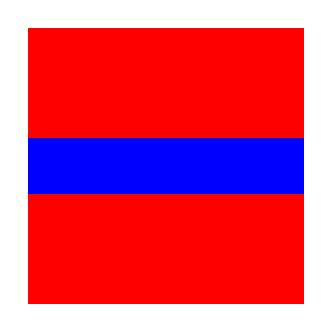
\begin{tikzpicture}[scale=0.7]
        \filldraw[draw=red, fill=red] (0,0) -- (0,5) -- (5,5) -- (5,0) -- cycle;
        \filldraw[draw=blue, fill=blue] (0,2) -- (0,3) -- (5,3) -- (5,2) -- cycle;
    \end{tikzpicture}
\end{figure}

\subsection{我就在那不动了——固定定位}

通过设置\lstinline|position: fixed|让一个元素固定在一个位置,它的相对移动的坐标是视图(屏幕内的网页窗口)本身。由于视图本身是固定的,它不会随着浏览器窗口的滚动条滚动而变化,除非在屏幕中移动浏览器窗口的屏幕位置,或改变浏览器窗口的显示大小。因此固定定位的元素会始终位于浏览器窗口内视图的某个位置,不会受文档流影响。

\begin{lstlisting}[style=htmlcssjs, title=固定定位, breaklines=true, breakatwhitespace=false]
<!DOCTYPE html>
<html lang="en">
<head>
    <meta charset="UTF-8">
    <title>固定定位</title>
    <style type="text/css">
        img {
            position: fixed;
            top: 15%;
            left: 20%;
        }
    </style>
</head>
<body>
    <img src="https://gimg2.baidu.com/image_search/src=http%3A%2F%2Fc-ssl.duitang.com%2Fuploads%2Fitem%2F201702%2F02%2F20170202151743_rvLWi.jpeg&refer=http%3A%2F%2Fc-ssl.duitang.com&app=2002&size=f9999,10000&q=a80&n=0&g=0n&fmt=jpeg?sec=1618588336&t=2612dc782456b9fdb8eeac0d0a215a85" alt="灰原哀.jpg" title="灰原哀">
    <br><br><br><br><br><br><br><br><br><br><br><br><br><br><br><br><br><br><br><br><br><br><br><br><br><br><br><br><br><br><br><br><br><br><br><br><br><br><br><br><br><br><br><br><br><br><br><br><br><br>
</body>
</html>
\end{lstlisting}

\mybox{奥运五环}

\begin{figure}[H]
    \centering
    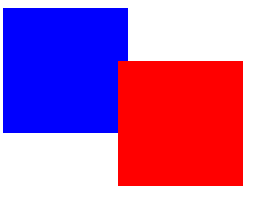
\includegraphics[scale=0.7]{img/C8/8-4/1.png}
\end{figure}

\begin{lstlisting}[style=htmlcssjs, title=olympic.html]
<!DOCTYPE html>
<html lang="en">
<head>
    <meta charset="UTF-8">
    <title>奥运五环</title>
    <link rel="stylesheet" type="text/css" href="olympic.css">
</head>
<body>
    <!-- 展示奥运五环的区域 -->
    <div class="stage">
        <div id="circle1"></div>
        <div id="circle2"></div>
        <div id="circle3"></div>
        <div id="circle4"></div>
        <div id="circle5"></div>
    </div>
</body>
</html>
\end{lstlisting}

\begin{lstlisting}[style=htmlcssjs, title=olympic.css]
* {
        margin: 0;
        padding: 0;
    }
    
    .stage {
        position: absolute;
        left: 50%;
        top: 50%;
        margin-left: -190px;
        margin-top: -93px;
        height: 185px;
        width: 380px;
    }
    
    #circle1,
    #circle2,
    #circle3,
    #circle4,
    #circle5 {
        position: absolute;
        width: 100px;
        height: 100px;
        border: 10px solid black;
        border-radius: 50%;
    }
    
    #circle1 {
        border-color: blue;
        left: 0;
        top: 0;
    }
    
    #circle2 {
        border-color: black;
        left: 130px;
        top: 0;
    }
    
    #circle3 {
        border-color: red;
        left: 260px;
        top: 0;
    }
    
    #circle4 {
        border-color: yellow;
        left: 65px;
        top: 70px;
    }
    
    #circle5 {
        border-color: green;
        left: 195px;
        top: 70px;
    }
\end{lstlisting}

\newpage